\documentclass[11pt]{article}
\usepackage{graphicx,listings}
\graphicspath{ {./images/} }
\title{\textbf{IoT 2023 Challenge 3}}
\author{
  Pasquale Castiglione\\
	\texttt{10657816}
  \and
  Lorenzo Campana\\
  \texttt{10605775}
}
\date{}
\begin{document}
\maketitle

\section{Introduction}
The goal of this challenge was to implement a routing algorithm in order to send a packet from Mote1 to Mote2.
\begin{figure}[h]
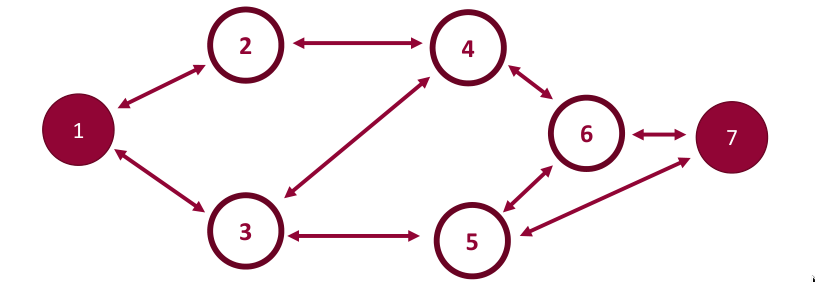
\includegraphics[width=\textwidth]{topology.png}
\caption{Network Topology}
\end{figure}
\section{Code}
\subsection{RadioRoute.h}
In the header file the data structures for the messages and for the routing table were defined.
\begin{lstlisting}[language=C]
typedef nx_struct radio_route_msg {
	nx_uint16_t type;
	nx_uint16_t sender;
	nx_uint16_t destination; // node_requested
	nx_uint16_t value; // cost
} radio_route_msg_t;
\end{lstlisting}

\begin{lstlisting}[language=C]
typedef struct route_entry_t {
	uint16_t next_hop;
  	uint16_t cost;
} route_entry_t;
\end{lstlisting}

\subsection{RadioRouteC.nc}
Two variables: \texttt{waiting\_packet} and \texttt{waiting\_address} were defined in order to store the message and the destination address to send when the routing table was empty.
At the beginning, right after the boot, the radio module was activated and a five seconds timer was started for the Mote 1.
\subsubsection{Send}
Before the sending of a message, the variabele \texttt{locked} is checked in order to check if the radio module is in use or not.
If the radio is free, 
\subsubsection{Receive}
Received messages are handled according to their type:
\begin{itemize}
	\item{\textbf{Data Message}}\\
		If the receiver node is not the intended destination then it checks if a route to the destination is present in its routing table.
		If a route is present then it forwards the message to the next hop.
	\item{\textbf{Route Request}}\\
		If the receiver node is the intended destination of a route request then it answers back sending a \texttt{Route Reply} broadcast message.
		Otherwise it broadcast again the route request message to its neighboors.
		
	\item{\textbf{Route Reply}}\\
		When a \texttt{Route Reply} is received the nodes check their routing table and update it if the recieved cost for the destination is lower than the stored one.  
\end{itemize}
\subsection{Led Control}
\section{Results}
\end{document}
